% cordillera-climate.tex
% ----------------------------------------------------------------------

% Copernicus-like latex2rtf compatible
\newif\iflatextortf
\iflatextortf
% copernicus_rtf.tex
% ------------------

% Base class and packages
\documentclass{article}
\usepackage{color}
\usepackage{geometry}
\usepackage{graphicx}
\usepackage{setspace}
\onehalfspacing

% Replacements for bibtex commands
\newcommand{\citep}[1]{(\textcolor{blue}{#1})}
\newcommand{\citet}[1]{\textcolor{blue}{#1}}

% Replacements for Copernicus commands
\newcommand{\introduction}[0]{\section{Introduction}}
\newcommand{\conclusions}[0]{\section{Conclusions}}
\newcommand{\tophline}[0]{\hline}
\newcommand{\middlehline}[0]{\hline}
\newcommand{\bottomhline}[0]{\hline}
\newcommand{\unit}[1]{\ensuremath{\mathrm{#1}}}
\newcommand{\degree}[0]{\ensuremath{^{\circ}}}

% Ignore other Copernicus commands
\newcommand{\runningtitle}[1]{}
\newcommand{\runningauthor}[1]{}
\newcommand{\received}[1]{}
\newcommand{\correspondence}[1]{}
\newcommand{\pubdiscuss}[1]{}
\newcommand{\revised}[1]{}
\newcommand{\accepted}[1]{}
\newcommand{\published}[1]{}


\else

% Copernicus manuscript
\documentclass[tc, manuscript]{copernicus}

% Copernicus final print
%\documentclass[tc]{copernicus}

% Copernicus discussion paper
%\documentclass[tcd, hvmath, online]{copernicus}
\fi

% Coloured hyperlinks
\hypersetup{hidelinks}

% Figure directory
\graphicspath{{figures/}}

% ----------------------------------------------------------------------
\begin{document}\hack{\sloppy}
% ----------------------------------------------------------------------

% Title
\title{The effect of climate forcing on numerical simulations of the Cordilleran ice sheet at the Last Glacial Maximum}

% Authors
\author[1]{J.~Seguinot}
\author[2]{C.~Khroulev}
\author[3]{I.~Rogozhina}
\author[1]{A.~P.~Stroeven}
\author[1]{Q.~Zhang}
\runningauthor{J.~Seguinot et~al.}
\correspondence{J.~Seguinot (julien.seguinot@natgeo.su.se)}

% Running title
\runningtitle{Climate forcing for Cordilleran ice sheet simulations}

% Affiliations
\affil[1]{Department of Physical Geography and Quaternary Geology and the Bolin Centre for Climate Research, Stockholm University, Stockholm, Sweden}
\affil[2]{Geophysical Institute, University of Alaska Fairbanks, Fairbanks, AK, USA}
\affil[3]{Helmholtz Centre Potsdam, GFZ German Research Centre for Geosciences, Potsdam, Germany}

% For Copernicus
\received{22~November 2013}
\accepted{5~December 2013}
\published{}

% Title
\firstpage{1}
\maketitle

% Abstract
\begin{abstract}
  We present an ensemble of numerical simulations of the Cordilleran ice sheet during the Last Glacial Maximum performed with the Parallel Ice Sheet Model (PISM), applying temperature offsets to the present-day climatologies from five different datasets. Monthly mean surface air temperature and precipitation from WorldClim, the NCEP/NCAR reanalysis, the ERA-Interim reanalysis, the Climate Forecast System Reanalysis and the North American Regional Reanalysis are used to compute surface mass balance in a~positive degree-day model. Modelled ice sheet outlines and volumes appear highly sensitive to the choice of climate forcing. For three of the four reanalysis datasets used, differences in precipitation are the major source for discrepancies between model results. We assess model performance against a~geomorphological reconstruction of the ice margin at the Last Glacial Maximum, and suggest that part of the mismatch is due to unresolved orographic precipitation effects caused by the coarse resolution of reanalysis data. The best match between model output and the reconstructed ice margin is obtained using the high-resolution North American Regional Reanalysis, which we retain for simulations of the Cordilleran ice sheet in the future.
\end{abstract}

% ----------------------------------------------------------------------
\introduction
\label{sec:intro}
% ----------------------------------------------------------------------

At the Last Glacial Maximum (LGM), glaciers of a~size comparable to the present Greenland and Antarctic ice sheets covered parts of Northern America (Laurentide, Cordilleran and Innuitian ice sheets) and northern Eurasia (Fennoscandian and Eurasian ice sheets). Numerical modelling of these former ice masses allows for a~comparison between glaciological theories embedded in the models and geomorphological traces underpinning palaeo-glaciological reconstructions. Yet, a~major obstacle in this exercise resides in large uncertainties concerning the climate forcing, typically atmospheric temperature and precipitation, required as input to numerical glacier models \citep{hebeler-etal-2008}. This includes uncertainty in the representation of Earth's present climate in regions of poor station coverage, and even larger uncertainty concerning accurate reconstructions of past climate change.

Arguably the most physically sound way to force an ice sheet model for simulations of glacial history is to couple it with a~General Circulation Model \citep[GCM;][]{yoshimori-etal-2001,calov-etal-2002,abeouchi-etal-2007,charbit-etal-2013}. However the computational demand of GCMs is such that only models of intermediate complexity can run on the time-scales of tens of thousands of years characteristic of ice sheet growth and decay.

Climatologies obtained from GCM palaeo-climate simulations such as produced within the Paleoclimate Modelling Intercomparison Project \citep[PMIP;][]{joussaume-taylor-1995} provide perhaps a~more reasonable representation of past climate. However, as such climatologies are only available for specific periods of time, using them as climate forcing for an ice sheet model requires either an assumption of steady-state ice sheet response to climatic fluctuations \citep{huybrechts-tsiobbel-1996}, or interpolation through time between climatologies from different periods, which can be linear \citep{charbit-etal-2002}, or modulated by a ``glacial index'' weighting function derived from ice core \chem{\delta^{18}O} records \citep{marshall-clarke-1999,tarasov-peltier-2004,zweck-huybrechts-2005,gregoire-etal-2012}. An important drawback in this approach is that GCM palaeo-climate simulations themselves rely on an accurate description of the global surface topography and therefore include global ice sheet reconstructions such as ICE-4G \citep{peltier-1994} for their surface topographic boundary condition. This condition could potentially exert influence on subsequently modelled ice sheet geometries, and particularly glacier extent.

However, avoiding this circular dependence requires simplifying assumptions regarding Earth's past climate. Such studies include energy balance modelling approaches \citep{tarasov-peltier-1997} and geographic parametrizations of surface mass balance \citep{robert-1991} or climate forcing \citep{johnson-fastook-2002}. Alternatively, temperature offset methods \citep{greve-etal-1999,bintanja-etal-2005} make use of the high level of detail available in present climate datasets such as gridded observation datasets, GCM output or reanalyses, while using simplifying representations of past climate deviations from the present state.

Here, we propose to address some of the uncertainties concerning climate forcing of numerical glacier models by evaluating the responses of a~numerical model, in terms of glacier extent, to inputs from several climate datasets. This is not entirely a~new approach as a~few studies of this kind are presently available. \citet{quiquet-etal-2012}, for example, assessed the sensitivity of a~Greenland ice sheet model to various climate forcing fields, including a~regional parametrization by \citet{fausto-etal-2009a}, output from several GCMs and an atmospheric reanalysis. \citet{rodgers-etal-2004} and \citet{charbit-etal-2007} tested the sensitivity of a~model of Northern Hemisphere ice sheets to climate forcing from different PMIP LGM simulations. Although using different set-ups, all three studies demonstrate the very large sensitivity of ice sheet models to the choice of climate forcing data used. To limit the degrees of freedom in our model and obtain results independent of palaeo-ice sheet reconstructions such as ICE-4G, we use a~simple temperature offset similar to the approaches by \citet{greve-etal-1999} and \citet{bintanja-etal-2005} and assess ice sheet model sensitivity to the choice of present-day climate data. Hence, rather than using GCM output, we force our model with climate reanalysis data, which builds on observational information through data assimilation \citep{bengtsson-etal-2007}. Furthermore, we focus our study regionally on the former Cordilleran ice sheet in western North America.

The Cordilleran ice sheet (Fig.~\ref{fig:locmap}) covered an area that presently experiences strong regional variations in climate. From a~numerical modelling perspective, it is one of the least studied palaeo-ice sheets of the Northern Hemisphere, despite the fact that significant stratigraphical, geomorphological, and chronological data is available to constrain its extent \citep{jackson-clague-1991,porter-swanson-1998,dukrodkin-1999,dyke-2004,kaufman-manley-2004,kleman-etal-2010,stroeven-etal-2010,stroeven-etal-inpress,margold-etal-2011}. The Cordilleran ice sheet has previously been modelled as part of efforts to simulate ice sheets in North America \citep{marshall-clarke-1999,calov-etal-2002,tarasov-peltier-1997,tarasov-peltier-2004,gregoire-etal-2012}, the Northern Hemisphere \citep{huybrechts-tsiobbel-1996,greve-etal-1999,charbit-etal-2002,charbit-etal-2007,charbit-etal-2013,johnson-fastook-2002,rodgers-etal-2004,bintanja-etal-2005,zweck-huybrechts-2005,abeouchi-etal-2007} and world-wide \citep{yoshimori-etal-2001}. While these studies generally reproduce the magnitude of North American glaciation at LGM reasonably well, there exists a~tendency in the simulations that are independent of ice sheet reconstructions such as the ICE-4G to predict excessive ice cover in parts of northern Yukon Territory and interior Alaska that have remained ice-free throughout the Pleistocene \citep{dukrodkin-1999,kaufman-manley-2004}.

Here we use PISM, a~Parallel Ice Sheet Model \citep{web:pism}, to simulate the extent and thickness of the Cordilleran ice sheet at the LGM (Fig.~\ref{fig:locmap}). We force our model with multiple climate datasets and compare the modelled ice extent to a~geomorphological reconstruction of the LGM ice sheet margin by \citet{dyke-2004}. We aim to determine the climate dataset which is most suited for simulation of the Cordilleran ice sheet and to use as input for future, transient studies over a~glacial cycle.

% ----------------------------------------------------------------------
\section{Model setup}
\label{sec:model}
% ----------------------------------------------------------------------

Given basal topography, sea level, geothermal heat flux and climate forcing, the model computes ice extent and thickness, its thermal and dynamic state, and the associated lithospheric response. Our modelling domain encompasses the entire area covered by the Cordilleran ice sheet at LGM including independent ice growing on the western Alaskan ranges and the Brooks Range and intermediate expanses of ice-free terrain in northern Yukon Territory and interior Alaska (Fig.~\ref{fig:locmap}).

As we aim to model glacial inception and growth of the Cordilleran ice sheet towards a~configuration as last attained during the LGM, we mimic palaeo-climatic conditions by applying constant temperature offsets homogeneously over the modelling domain. Each simulation starts from ice-free conditions and runs for 10\,kyr, a~time interval representative of the rapid build-up of the last Cordilleran ice sheet from nearly ice-free to full glacial conditions \citep{clague-1989,stroeven-etal-2010}. Our simulations are performed in parallel on 32 cores at the Swedish National Supercomputing Center.

\subsection{Ice thermodynamics}

The central part of an ice sheet model consists of the computation of flow velocity which itself depends on temperature. PISM is a~shallow model, which implies that the balance of stresses is approximated based on their predominant components. On the other hand, the model is polythermal: it accounts for differences in temperature and softness within the ice column.

The Shallow Shelf Approximation (SSA) is used as a ``sliding law'' for the Shallow Ice Approximation (SIA) \citep{bueler-brown-2009,winkelmann-etal-2011}. SIA and SSA velocities are computed by finite difference methods on a~10\,km resolution horizontal grid of 300 by 150 points (the modelling domain). Ice softness depends on temperature and water content through an enthalpy formulation \citep{aschwanden-blatter-2009,aschwanden-etal-2012}. Enthalpy is computed in three dimensions in up to 51 irregularly spaced layers within the ice, and temperature is additionally computed in 11 regularly spaced layers in bedrock to a~depth of 1\,km. Surface air temperature from the climate forcing provides the upper boundary condition to the ice enthalpy model, and a~geothermal heat flux of 70\,\unit{mW\,m^{-2}} provides the lower boundary condition to the bedrock thermal model. Although this uniform value does not account for the high spatial geothermal variability in the region, it is on average representative of available heat flow measurements \citep{artemieva-mooney-2001,blackwell-richards-2004}. Whereas spatial variations in the geothermal heat flux may significantly affect basal conditions \citep{pattyn-2010}, this study focuses on reconstructing the former extent of the Cordilleran ice sheet, on which it has relatively little effect \citep{rogozhina-etal-2012}.

A~pseudo-plastic sliding law \citep{aschwanden-etal-2013} relates the bed-parallel shear stress and the sliding velocity. The yield stress is modelled using the Mohr--Coulomb criterion. The till friction angle $\phi$ varies from 10 to 30{\degree}. It is computed once at the beginning of the run, as a~function of modern bed elevation, with lowest values occurring at low elevations,

\begin{align}
  \phi =
  \begin{cases}
    10      & \text{for }       z<  0 \\
    z/10+10 & \text{for }    0 <z<200 \\
    30      & \text{for }  200 <z     \\
  \end{cases}
\end{align}

where $\phi$ is given in degrees and $z$ in meters above current sea level. This model thus accounts for a~weakening of till associated with the presence of marine sediments \citep{martin-etal-2011,aschwanden-etal-2013}. Because the distribution of marine sediments is assumed constant throughout the run, the till friction angle $\phi$ is not affected by changes in bed elevation. Basal topography (Fig.~\ref{fig:topo}) is derived from the ETOPO1 combined topography and bathymetry dataset with a~resolution of 1\,arc-min \citep{data:etopo1}.

Sea level is lowered by 120\,m and basal topography responds to ice load following a bedrock deformation model that includes point-wise isostasy, elastic lithosphere flexure and viscous mantle deformation in a~semi-infinite half-space \citep{lingle-clark-1985,bueler-etal-2007}. It uses a lithosphere density of 3300\,\unit{kg\,m^{-3}}, a flexural rigidity of $5 \times 10^{24}$\,\unit{N\,m} and a mantle viscosity of $1 \times 10^{21}$\,\unit{Pa\,s}. Due to the high mantle viscosity, there exists a time lag between ice sheet growth and isostatic bedrock response.

\subsection{Surface mass-balance}

Ice surface accumulation and ablation are computed from monthly mean surface air temperature and monthly precipitation by a~temperature-index (positive degree-day) model \citep{hock-2003}. Ice accumulation is equal to precipitation when temperature is below 0\,\unit{{\degree}C}, and decreases to zero linearly with temperature between 0 and 2\,\unit{{\degree}C}. Ice ablation is computed from the number of positive degree-days, defined as the integral of temperatures above 0\,\unit{{\degree}C} in one year. 

The positive degree-day integral \citep{calov-greve-2005} is numerically approximated using week-long sub-intervals. It accounts for temperature variability assuming a~normal distribution along a~central (input) value. The temperature standard deviation is a~constant model parameter and was assigned a~value of 3.07\,\unit{{\degree}C}, which corresponds to the mean summer (JJA), model domain-averaged monthly standard deviation of daily mean temperature from monthly mean temperature, as computed from North American Regional Reanalysis data \citep{data:narr} in a~manner similar to \citet{seguinot-2013}. The ablation model incorporates degree-day factors of 3.04\,\unit{mm\,{\degree}C^{-1}\,day^{-1}} for snow and 4.59\,\unit{mm\,{\degree}C^{-1}\,day^{-1}} for ice, as derived from mass-balance measurements on contemporary glaciers from the Coast Mountains and Rocky Mountains in British Columbia \citep{shea-etal-2009}.

\subsection{Air temperature corrections}

Prior to surface mass balance computation, the model dynamically applies a~lapse-rate correction to surface air temperature. This correction accounts for the evolution of ice thickness on the one hand, and differences between the climate forcing reference topography and the ice flow model basal topography on the other hand. It uses a~reference topography distinct from the modelled basal topography and specific to each climate forcing dataset (Fig.~\ref{fig:topo}). An annual lapse rate of 6\,\unit{{\degree}C\,km^{-1}} is used in all simulations. No corrections apply to precipitation changes with elevation.

% ----------------------------------------------------------------------
\section{Climate forcing}
\label{sec:climate}
% ----------------------------------------------------------------------

Our climate forcing consists of monthly climatologies of surface air temperature and precipitation obtained from one observational dataset, three global reanalyses and one regional reanalysis.

\subsection{Observational data: WorldClim}

WorldClim is a~high resolution global climate dataset built from meteorological observations \citep{data:worldclim}. It was built by applying a~spatial interpolation between a~large set of measurements taken at terrestrial weather stations worldwide, using SRTM \citep{data:srtm} and GTOPO30 elevation data \citep{data:gtopo30}. This dataset provides a~resolution much higher than attained by circulation models, however its reliability is variable due to the highly inhomogeneous distribution of measurements \citep{data:worldclim}.

Within our modelling domain, the spatial distributions of summer (JJA) and winter (DJF) air surface temperatures in WorldClim generally show a~decrease of temperature from south to north (JJA) and from south-west to north-east (DJF), such that regions further inland experience colder winters (Fig.~\ref{fig:temp}). It should be noted that temperature gradients are much stronger in winter than in summer. Temperature rises well above zero during the summer months over the entire modelling domain, except for the highest mountain peaks, and even regions where mean annual temperatures are well below freezing point do experience warm summers. In other words, there is a~strong contrast in seasonality between coastal temperate-climate and inland continental-climate regions.

The spatial distribution of JJA and DJF mean precipitation rates in WorldClim reveals a~strong precipitation decline beyond the coastal regions (Fig.~\ref{fig:prec}), primarily as a~result of the continuous orographic barrier formed by the Wrangell and St.-Elias mountains, the Coast Mountains and the Cascades (Fig.~\ref{fig:locmap}). A~less pronounced precipitation peak is also visible over the interior ranges. From an ice sheet mass balance point of view, these heterogeneities become even stronger due to the difference in timing of the precipitation peak through the year. Whereas coastal regions experience most precipitation as snow during the accumulation season (DJF), inland regions experience dry winters and most of the annual precipitation consequently falls as rain during the ablation season (JJA).

In regions such as the northern Yukon Territory and interior Alaska, dry winters and warm summers prohibit ice to accumulate and glaciers to form, despite strongly negative mean annual temperatures. In order to account for these strong gradients in seasonality, we use monthly rather than annual averages of temperature and precipitation to drive the ice sheet model.

There are two problems inherent to the use of WorldClim data in our study area. Firstly, the density of weather stations used by WorldClim in the Northern American Cordillera is highly inhomogeneous. Although good coverage exists for the southern part of our modelling domain, several hundred kilometres can separate neighbouring stations in the north \citep{data:worldclim}. Secondly, WorldClim lacks data offshore, which would have been particularly useful over the Pacific continental shelf which was partly covered by ice during the LGM \citep{jackson-clague-1991}.

\subsection{Reanalysis data: NCEP/NCAR, ERA-Interim, CFSR and NARR}

In addition to the WorldClim data, we use surface air temperatures and precipitation rates from three global atmospheric reanalyses and one regional atmospheric reanalysis to inform the mass balance routine of PISM: the NCEP/NCAR reanalysis \citep{data:ncar}, the ERA-Interim reanalysis \citep{data:erai}, the Climate Forecast System Reanalysis \citep[CFSR;][]{data:cfsr}, and the North American Regional Reanalysis \citep[NARR;][]{data:narr}. Monthly climatologies from NCEP/NCAR and NARR reanalyses were provided by the \citet{web:psd} whereas monthly climatologies from the ERA-Interim and CFSR reanalyses were computed from their monthly mean time series (Table~\ref{tab:reanalyses}).

The spatial distributions of JJA air surface temperatures and DJF precipitation rates from the four reanalysis climatologies are shown in Figs.~\ref{fig:temp} and~\ref{fig:prec}. Summer temperature and winter precipitation are most relevant to the glacier model as they drive summer melt and winter accumulation, respectively. Because reanalyses include observational information through data assimilation, they are closer to observations than pure GCMs in densely monitored regions, such as the southern part of our modelling domain \citep{bengtsson-etal-2007}. On the other hand, the atmospheric physics embedded in the models provide more realistic output than obtained by spatial interpolation in sparsely monitored regions, such as the northern part of our modelling domain.

\subsection{Preprocessing and lapse-rate corrections}

WorldClim, NCEP/NCAR, ERA-Interim, CFSR and NARR climatologies were re-projected to the Canadian Atlas Lambert conformal conic projection (EPSG code~3978) and bilinearly interpolated to the 10\,km resolution model grid using the module r.proj from GRASS~GIS \citep{soft:grass}. In addition, WorldClim data was extrapolated to cover grid points in the ocean using the nearest-neighbour algorithm \citep{soft:scipy}. Note that here we choose to present original rather than interpolated data, in order to highlight differences between datasets related to spatial resolution (Figs.~\ref{fig:temp} and~\ref{fig:prec}).

The CFSR climatology presents wave-like artefacts in its precipitation field (Fig.~\ref{fig:prec}). These are a~common feature in GCM simulations due to the failure of spectral models to resolve the very local nature of topography-induced precipitation events, which becomes particularly visible in the high-resolution, less spatially-smoothed data. Therefore, an alternative forcing was prepared for CFSR by smoothing its precipitation field. This was achieved by averaging data locally in a~circular kernel of 7\,pixels in diameter prior to re-projection using the module r.neighbors from GRASS~GIS \citep{soft:grass}. Finally, input files for PISM were prepared using \citet{web:nc4py}.

% ----------------------------------------------------------------------
\section{Results}
\label{sec:results}
% ----------------------------------------------------------------------

Using WorldClim, NCEP/NCAR, ERA-Interim, CFSR (smoothed and original datasets) and NARR input climatologies as climate forcing, we run 66~simulations of glacial inception and growth of the Cordilleran ice sheet over 10\,kyr using temperature offsets ranging from -10 to 0\,\unit{{\degree}C}. Significant differences in patterns of ice sheet growth, final glacial extent, and volume are attained (Figs.~\ref{fig:ivolarea}--\ref{fig:cool05}).

Across the range of temperature offsets used, final glaciated area and final ice volume differ widely between different input climatologies (Fig.~\ref{fig:ivolarea}). For instance, using a~-5\,\unit{{\degree}C} temperature offset, final glaciated area differs between WorldClim and CFSR forcing by a~factor of~6 and final volume by a~factor of~12 (Fig.~\ref{fig:ivolarea}). For particular temperature offset values, given input climatologies result in similar final glaciated areas and ice volumes, yet regional patterns are different (Fig.~\ref{fig:extent}).

Under present climate (0\,\unit{{\degree}C} offset), WorldClim, ERA-Interim and NARR forcing produce local ice caps in areas presently glaciated (Fig.~\ref{fig:extent}). These results are fairly consistent with contemporary ice distribution, although both the 10\,\unit{km} horizontal resolution and the occurrence of glaciers and ice caps surface topographies in the ETOPO1 dataset used for basal topography prevent a~meaningful detailed comparison. CFSR forcing, on the other hand, yields continuous ice cover over the northern Coast Mountains, and NCEP/NCAR forcing results in ice sheet growth, both of which are largely inconsistent with the present state of glaciation. At the opposite side of the temperature offset range, it can be noted that both the NCEP/NCAR and CFSR forcing produce oversized ice sheets whose extents are primarily restricted by the domain boundaries (Fig.~\ref{fig:extent}). The smoothing of CFSR precipitation yields an insignificant effect on the resulting ice sheet geometry.

To contrast the effect of the six different input climatologies, we plot simulations using a~-5\,\unit{{\degree}C} temperature offset (Fig.~\ref{fig:cool05}). The magnitude of glaciation differs dramatically from one climate forcing to another. Whereas the NCEP/NCAR and CFSR climatologies produce a~large ice sheet that covers most of the model domain (Fig.~\ref{fig:cool05}, lower panels), WorldClim, ERA-Interim and NARR climatologies lead to a~more restrictive ice cover (Fig.~\ref{fig:cool05}, upper panels). The WorldClim run only resulted in the growth of mountain ice caps bounded to the highest topography.

% ----------------------------------------------------------------------
\section{Discussion}
\label{sec:discussion}
% ----------------------------------------------------------------------

These simulations of the LGM Cordilleran ice sheet show a~very large sensitivity to the choice of climate forcing data used (Figs.~\ref{fig:ivolarea}--\ref{fig:cool05}). To understand the origin of the discrepancies between model results, we quantify differences in surface air temperature and precipitation rate between the input climatologies and test their effect on the ice sheet model. We then compare our findings to a~geomorphological reconstruction of the LGM Cordilleran ice sheet margin, and discuss some of the key assumptions of this study.

\subsection{Comparison of forcing climatologies}

As previously outlined, significant differences in the distribution of winter (DJF) precipitation and summer (JJA) temperature, which are the predominant controls on accumulation and melt at the modelled ice sheet surface, exist between datasets (Figs.~\ref{fig:topo}--\ref{fig:prec}). In this section we use the WorldClim climatology, which is derived from observations, as a~reference with which to compare other climate forcing data on land.

Because much of the disparity between reanalyses and observational temperature data is caused by topographical detail at scales unresolved in the reanalyses, we apply a lapse-rate correction prior to this comparison, using the same lapse rate of 6\,\unit{{\degree}C\,km^{-1}} as in the simulations. ERA-Interim, CFSR and NARR climatologies exhibit temperature distributions fairly consistent with WorldClim data (Fig.~\ref{fig:tempheatmap}). The spatial distribution of temperature differences between reanalyses and WorldClim data shows partly consistent patterns, such as positive anomalies in the northernmost part of the modelling domain. These may relate to weaknesses of WorldClim data in areas of sparse observational coverage (Fig.~\ref{fig:tempdiff}). However, significant disparity among reanalyses exists, too. More specifically, surface air temperature data from the NCEP/NCAR climatology shows the largest disparity with that of WorldClim, with a~significant cold anomaly over most of the modelling domain (Figs.~\ref{fig:tempheatmap} and \ref{fig:tempdiff}).

All four reanalyses used in this study exhibit higher precipitation rates than WorldClim data (Fig.~\ref{fig:precheatmap}). However the magnitude of this anomaly differs significantly between datasets. The spatial distributions of precipitation differences between reanalyses and WorldClim data show that negative precipitation anomalies are generally constrained to the windward slope of the major mountain ranges, while positive precipitation anomalies are found on the leeward slope of these ranges and extend downwind to interior plateaux and lowlands (Fig.~\ref{fig:precdiff}).

Most likely, this is the signature of an orographic precipitation effect. The topography of the Northern American Cordillera is such that its western ranges form a~continuous orographic barrier, causing high precipitation along the Pacific coast while leaving much of the interior arid. The ability of a~GCM to reproduce these contrasts in precipitation is bounded by spatial resolution. In a~model of coarser resolution, these high mountain ranges are reduced to smooth hills and the modelled distribution of precipitation is also smoother (Fig.~\ref{fig:oroprecip}). However, this effect alone cannot explain the widespread and pronounced positive precipitation anomalies observed in CFSR data (Figs.~\ref{fig:precheatmap} and \ref{fig:precdiff}) despite its high spatial resolution (Table~\ref{tab:reanalyses}).

\subsection{Model sensitivity to climate forcing}

To distinguish the effects of temperature and precipitation biases on the ice sheet model, we run a~series of eight additional simulations. These new simulations use a ``hybrid'' climate forcing that consists of temperature data from WorldClim, combined with precipitation data from each of the four reanalyses, and vice-versa. A~single temperature offset of -5\,\unit{{\degree}C} is used. This value was chosen to allow for comparison with previous results (Fig.~\ref{fig:cool05}). In each case, temperature lapse rates are computed using the reference topography from the corresponding dataset.

Although only temperature or precipitation changes are applied, this experiment results once more in large differences in modelled ice sheet geometries (Fig.~\ref{fig:biatm}) as compared to the reference WorldClim -5\,\unit{{\degree}C} run (Fig.~\ref{fig:cool05}, top-left panel). For ERA-Interim, CFSR and NARR climatologies, precipitation anomalies clearly dominate the differences in ice sheet response, whereas temperature anomalies have relatively little effect (Fig.~\ref{fig:biatmbars}). However, in the case of NCAR forcing, both the negative temperature bias (Figs.~\ref{fig:tempheatmap} and \ref{fig:tempdiff}) and the important precipitation differences (Figs.~\ref{fig:precheatmap} and \ref{fig:precdiff}) contribute approximately equally to produce oversized ice sheets (Fig.~\ref{fig:biatmbars}).

\subsection{Comparison to geomorphological LGM margin reconstruction}

We compare modelled ice sheet geometries to a~reconstruction of the ice margin at 14\,\unit{\chem{^{14}C}\,kyr\,BP} (16.8\,cal\,kyr\,BP) by \citet{dyke-2004}, based on glacial geomorphology and radiocarbon dating (Fig.~\ref{fig:locmap}). This corresponds to the LGM extent of most of the Cordilleran ice sheet, which occurred later than for the Laurentide ice sheet \citep{porter-swanson-1998,dyke-2004,stroeven-etal-2010,stroeven-etal-inpress}.

Considering previously identified weaknesses of the CFSR and NCEP/NCAR data (Figs.~\ref{fig:tempheatmap}--\ref{fig:biatmbars}), we restricted our analysis to the WorldClim, ERA-Interim and NARR input climatologies. In order to compare modelled ice sheets of a~similar size, we select for each climate forcing the simulation that leads to a~final glaciated area closest to the approximate size of the LGM Cordilleran ice sheet of $2\times 10^6\,\unit{km^2}$. This corresponds to temperature offset values of -8\,\unit{{\degree}C} (WorldClim), -6\,\unit{{\degree}C} (ERA-Interim) and -7\,\unit{{\degree}C} (NARR). These qualitative ``best'' runs are presented in Fig.~\ref{fig:best} along with their associated temperature depressions and a~reconstruction of the LGM ice sheet margin by \citet{dyke-2004}.

Although this selection results in similarly sized ice sheets, noticeable differences in shape exist. The ERA-Interim simulation produces a~more northerly-centred ice sheet with too much ice in the north and too little in the south. This may partly reflect unresolved orographic precipitation effects (Fig.~\ref{fig:oroprecip}) due to the coarser GCM resolution (Table~\ref{tab:reanalyses}). The LGM ice sheet margin by \citet{dyke-2004} is best reproduced by simulations driven by input climatologies from WorldClim and NARR data. However, common discrepancies between the modelled ice sheet geometry and the geomorphological reconstruction can still be observed (Fig.~\ref{fig:best}).

Firstly, the modelled eastern margin of the ice sheet extends further east than the inferred position of the junction between the Cordilleran and the Laurentide ice sheets. This can be seen for instance in the south-eastern part of our modelling domain, where the modelled ice sheets cover an ice-free corridor of the LGM reconstruction (Fig.~\ref{fig:best}). However, such comparisons have been hampered by the fact that we have not considered the buttressing effect of the Laurentide ice sheet, which would have inhibited the Cordilleran ice sheet from advancing onto the Canadian Prairies. In addition, potential effects of the growing ice-sheet on atmospheric circulation and precipitation changes are not included in our model. The Cordilleran ice sheet initiated from the formation of mountain ice caps over the high mountain ranges \citep{clague-1989}. In our simulations, a~continuous ice cover quickly forms over the western ranges, where precipitation rates are higher than in the rest of the domain. In reality, this continuous ice cover enhanced the topographical barrier already formed by the western ranges, and would have resulted in less precipitation and warmer air in the interior. This process of ``self-inhibiting growth'' is not captured in our model but was demonstrated to be important in a~similar setting over Greenland, where it may have been limiting the advance of the ice sheet during its build-up \citep{langen-etal-2012}.

Secondly, our simulations produce anomalous ice cover on parts of the continental shelf in the Arctic Ocean (Fig.~\ref{fig:best}). These regions experience a~marine climate, including lower summer temperature than on the adjacent land (Fig.~\ref{fig:temp}). However in our simulations, sea-level is lowered by 120\,\unit{m}, turning large parts of the low-sloping continental shelf into land. This anomalous ice cover is to be interpreted as an artefact arising from our simplistic temperature offset method, and has little effect on the rest of the results.

Given the lack of WorldClim data offshore, we consider the NARR climate forcing as best suited for simulations of the Cordilleran ice sheet among those tested, and under the assumptions of the present study.

\subsection{Model sensitivity to the duration of ice sheet inception}

Most of the simulations presented in this study, and more particularly those that reproduce the LGM ice margin reconstruction more closely (Fig.~\ref{fig:best}) do not reach a steady-state. Instead, rates of growth remain high throughout the run, and bed elevation does not come close to equilibrium with the ice load. In turn, a~key assumption for the present study is our choice of 10\,kyr for the duration of all our simulations. Although geomorphological data shows that the period of Cordilleran ice sheet inception, from nearly ice-free to full glacial conditions, could not have been much longer than 10\,kyr, they provide no lower bound to this value.

To test the effect of an inception period of shorter duration on model results, we use simulations run under NARR climate forcing with temperature offsets of -11 to -7\,\unit{{\degree}C}, and compare modelled ice sheet extent when glaciated area reaches the approximate size of the LGM Cordilleran ice sheet of $2\times 10^6\,\unit{km^2}$.

This experiment shows that a~shorter start-up period leads to more restricted ice cover in the eastern part of the modelling domain, where precipitation rate controls ice advance, but more extensive glaciation in the south-western domain along the Pacific coast, where temperature is the limiting factor (Fig.~\ref{fig:durationstack}). Hence, reducing simulation duration leads to a~closer match with the LGM ice sheet margin by \citet{dyke-2004} in some sectors of the modelling domain, but higher discrepancy in other sectors.

\subsection{Other potential method improvements}

Our representation of climate history by constant temperature offsets is voluntarily simplistic. To better understand the transient character of the LGM Cordilleran ice sheet, time-dependent palaeo-climate forcing would be needed. Although it is clear that past temperature changes over the region were neither homogeneous nor constant in time, their patterns are not trivial and may potentially display a~strong inter-dependence with the evolution of the Cordilleran and Laurentide ice sheets. As previously discussed, potential effects of the growing ice-sheet on precipitation changes are not included in our model. These changes likely consisted of a reduction of precipitation in continental regions and in the ice sheet interior, and an increase of precipitation along part of the margin where the presence of ice imposed ascending winds. They could result in a more westerly-centred ice sheet than modelled here, with lower ice thickness in its interior. In addition, the final position of the eastern ice margin is largely controlled by its advance rate through the run. Therefore, the precipitation shadowing effects may have resulted in more similar ice-sheet configurations if they were included in the model. Although using a GCM of intermediate complexity \citep{yoshimori-etal-2001,calov-etal-2002,abeouchi-etal-2007,charbit-etal-2013} may represent a first step towards including ice sheet feedback on climate, their spatial resolution does not allow for accurate modelling of orographic precipitation changes in a region as mountainous as the North American Cordillera.

Furthermore, the surface mass balance model crudely simplifies the processes taking place at the glacier surface. Refreezing of melted snow and ice and water retention in the snow pack was shown to influence surface mass balance of glaciers \citep{trabant-mayo-1985}, yet it is not accounted for in our PDD model. Based on scarce observations over the Greenland ice sheet, different parametrizations of this effect have been developed \citep{janssens-huybrechts-2000,fausto-etal-2009b}. However, these parametrizations were shown to disagree with more complex models \citep{reijmer-etal-2012}, and it remains undemonstrated whether their application to a~different region and time period is sound. In addition, we simulate temperature variability by using a~constant, uniform value of daily temperature standard deviation. This approach implies large biases of surface mass-balance \citep{charbit-etal-2013,rogozhina-rau-2014,seguinot-2013}, particularly over regions with such various climates as experienced within our model domain.

The bedrock deformation model uses homogeneous lithospheric properties and a semi-infinite mantle of constant viscosity. Thus, it does not represent lateral variations of crustal and mantle properties characteristic of tectonically active margins such as the American Cordillera, nor does it include the influence from the neighbouring Laurentide ice sheet. These limitations should be acknowledged when interpreting ice surface elevation and volume reconstructions presented in this study.

% ----------------------------------------------------------------------
\conclusions
\label{sec:concl}
% ----------------------------------------------------------------------

Our study shows a~strong dependency of ice sheet model results on the choice of climate forcing data. For three of the four reanalysis datasets used, precipitation rate, over surface air temperature, causes much of the variation in modelled ice sheet outlines and volumes. Furthermore, the spatial resolution of input data appears critical for providing the ice sheet model with an accurate precipitation field, confirming results obtained by \citet{quiquet-etal-2012} from various GCM forcing datasets over the Greenland ice sheet.

For the Cordilleran ice sheet, we achieve the best fit to the mapped LGM margin by \citet{dyke-2004} using climate forcing from the high-resolution interpolated observational dataset WorldClim \citep{data:worldclim} and the North American Regional Reanalysis \citep[NARR;][]{data:narr}. The latter dataset is preferable in our case due to the lack of WorldClim data offshore. Climate forcing from CFSR and the NCEP/NCAR reanalysis produce largely oversized ice sheets due to too high precipitation rates, and in the second case, too low surface air temperature. The ERA-Interim data used in this study produces more reasonable results, but it may be too coarse to accurately resolve the spatial distribution of orographic precipitation associated with the rugged topography of the study area, resulting in a~misplaced ice coverage in regard to geomorphological data. Therefore, we retain NARR data for forcing simulations of the Cordilleran ice sheet in the future.

One must keep in mind, however, that these results are only accurate for our choices of ice-sheet model (PISM), surface mass balance model (PDD), study object (the Cordilleran ice sheet), and, most importantly, palaeo-climate representation (temperature offsets). At LGM, it is most likely that the presence of ice sheets significantly affected circulation patterns and distribution of precipitation. At the cost of greater computational expense, a~more accurate representation of palaeo-climate may allow for a~better fit between model results and the mapped LGM margin.

% Acknowledgements
\begin{acknowledgements}
  We thank Ed Bueler and Andy Aschwanden for providing constant support on PISM and patiently answering our questions on the code internals, Laurent Brodeau and Soon-Heum Ko for assistance concerning software installations on supercomputing resources, and all PISM authors for providing the model open-source. This work was supported by the Swedish Research Council (VR) grant {\#}2008-3449 to A. P. Stroeven and by NASA grant {\#}NNX13AM16G to E. Bueler. Computer resources were provided by the Swedish National Infrastructure for Computing (SNIC) allocation {\#}2013/1-145 to A. P. Stroeven at the National Supercomputing Center (NSC).\\ 

  % Author contributions
  \hack{\noindent}\textit{Author contributions.}
J. Seguinot ran the simulations and wrote most of the paper; C. Khroulev implemented necessary code changes in PISM; I. Rogozhina helped with model set-up and experiment design; A. P. Stroeven initiated the Cordilleran ice sheet modelling project; and Q. Zhang prepared some of the forcing data. All authors contributed to paper writing.
\end{acknowledgements}

% References
\input{references.bbl}
\newpage

% ----------------------------------------------------------------------
% Floats
% ----------------------------------------------------------------------

% tab:reanalyses
\begin{table*}[t]
  \caption{Characteristics of reanalysis climatologies used to inform the mass balance component of PISM.}
  \label{tab:reanalyses}
  {\begin{tabular}{lcccc}
    \tophline
    Reanalysis& Spatial coverage& Averaging period& Resolution& Description\\
    \middlehline
    NCEP/NCAR   & global        & 1981--2010 & 1.875{\degree} & \citet{data:ncar} \\
    ERA-Interim & global        & 1979--2011 & 1.000{\degree} & \citet{data:erai} \\
    CFSR        & global        & 1979--2010 & 0.325{\degree} & \citet{data:cfsr} \\
    NARR        & North America & 1979--2000 & 32\,km       & \citet{data:narr} \\
    \bottomhline
  \end{tabular}}
  \belowtable{}
\end{table*}

% fig:locmap
\begin{figure}
  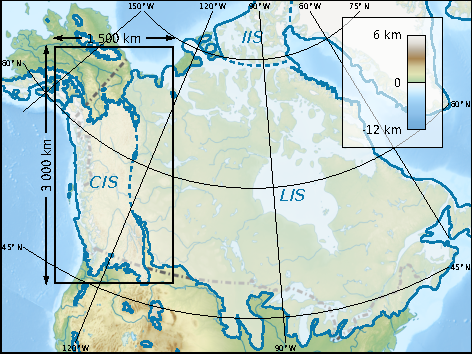
\includegraphics[width=80mm]{cordillera-climate-locmap}
  \caption{Shaded relief map of northern North America with the extent of the Cordilleran (CIS), Laurentide (LIS) and Innuitian (IIS) ice sheets at 14\,\unit{\chem{^{14}C}\,kyr\,BP} (16.8\,cal\,kyr\,BP) \citep{dyke-2004}. While this age denotes the LIS after retreat from its LGM, it closely corresponds to the LGM extent of most of the Cordilleran ice sheet \citep{porter-swanson-1998,dyke-2004,stroeven-etal-2010}. The rectangular box denotes the modelling domain of the Cordilleran ice sheet of 1500 by 3000\,km. Major mountain ranges covered by the ice sheet include the Wrangell and St.-Elias mountains (W--SE), the Selwyn and MacKenzie mountains (S--MK), the Coast Mountains and the Rocky Mountains. The background map consists of ETOPO1 \citep{data:etopo1} and Natural Earth Data \citep{data:naturalearth} and was assembled with GRASS~GIS \citep{soft:grass}.}
  \label{fig:locmap}
\end{figure}

% fig:topo
\begin{figure*}
  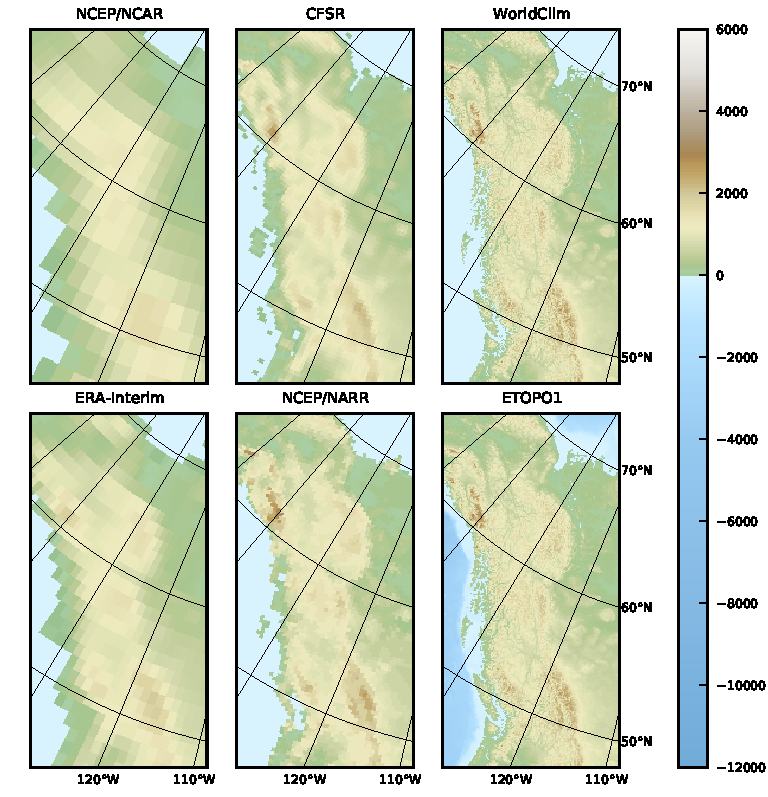
\includegraphics{cordillera-climate-topo}
  \caption{Topography maps from WorldClim \citep{data:worldclim}, ERA-Interim reanalysis \citep{data:erai}, North American Regional Reanalysis \citep[NARR;][]{data:narr}, ETOPO1 \citep{data:etopo1}, Climate Forecast System Reanalysis \citep[CFSR;][]{data:cfsr}, and NCEP/NCAR reanalysis \citep{data:ncar}. Whereas ETOPO1 is used as basal topography for the ice sheet model, all other data are used as a~reference for temperature lapse-rate corrections. Figs.~\ref{fig:topo}--\ref{fig:durationstack} are drawn using Matplotlib \citep{soft:mpl}.}
  \label{fig:topo}
\end{figure*}

% fig:temp
\begin{figure*}
  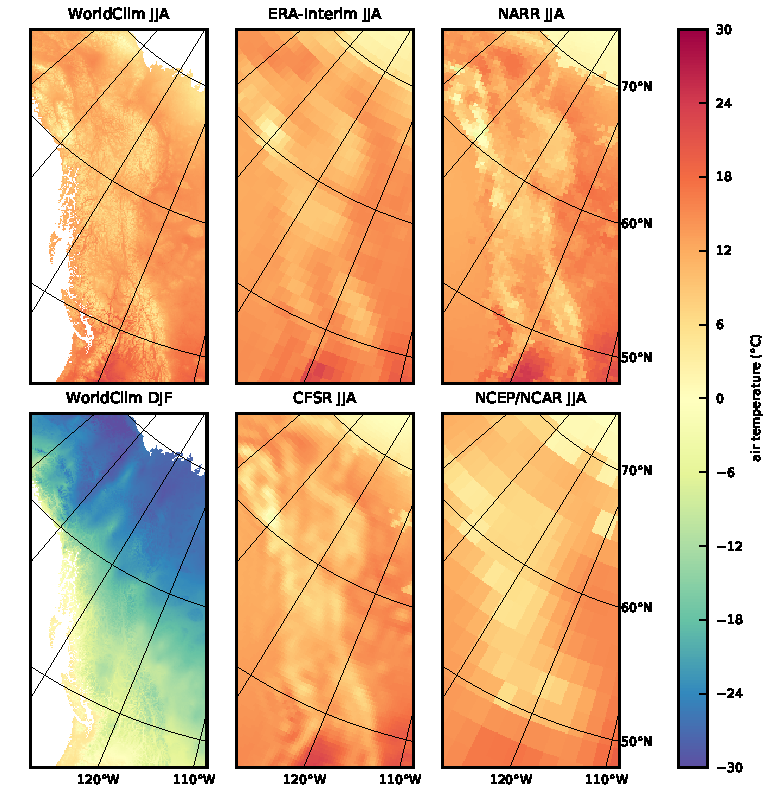
\includegraphics{cordillera-climate-temp}
  \caption{Summer (JJA) and winter (DJF) temperature maps from WorldClim \citep{data:worldclim}, and summer (JJA) temperature maps from ERA-Interim reanalysis \citep{data:erai}, North American Regional Reanalysis \citep[NARR;][]{data:narr}, Climate Forecast System Reanalysis \citep[CFSR;][]{data:cfsr}, and NCEP/NCAR reanalysis \citep{data:ncar} climatologies.}
  \label{fig:temp}
\end{figure*}

% fig:prec
\begin{figure*}
  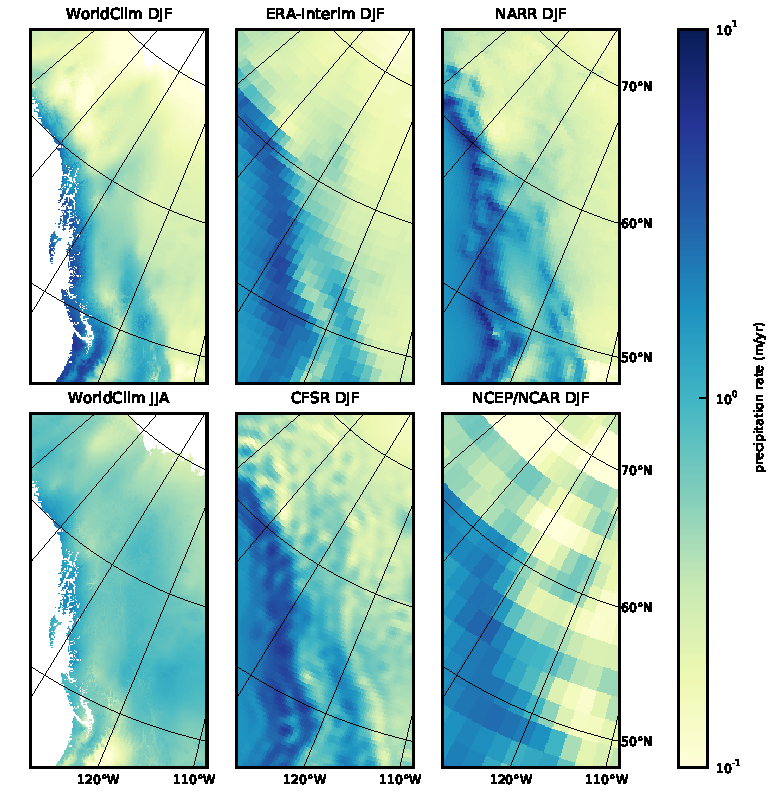
\includegraphics{cordillera-climate-prec}
  \caption{Winter (DJF) and summer (JJA) precipitation maps from WorldClim \citep{data:worldclim}, and winter (DFJ) temperature maps from ERA-Interim reanalysis \citep{data:erai}, North American Regional Reanalysis \citep[NARR;][]{data:narr}, Climate Forecast System Reanalysis \citep[CFSR;][]{data:cfsr}, and NCEP/NCAR reanalysis \citep{data:ncar} climatologies. Additional forcing data was prepared to correct for wave-like precipitation artefacts in CFSR (Sect.~\ref{sec:climate}).}
  \label{fig:prec}
\end{figure*}

% fig:ivolarea
\begin{figure}
  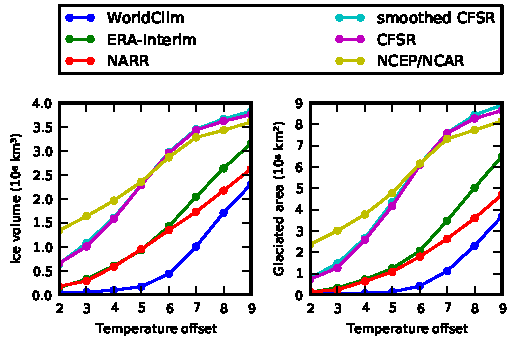
\includegraphics{cordillera-climate-ivolarea}
  \caption{Total glaciated area and ice volume after 10\,kyr as a~function of temperature offset for each climate forcing used.}
  \label{fig:ivolarea}
\end{figure}

% fig:extent
\begin{figure*}
  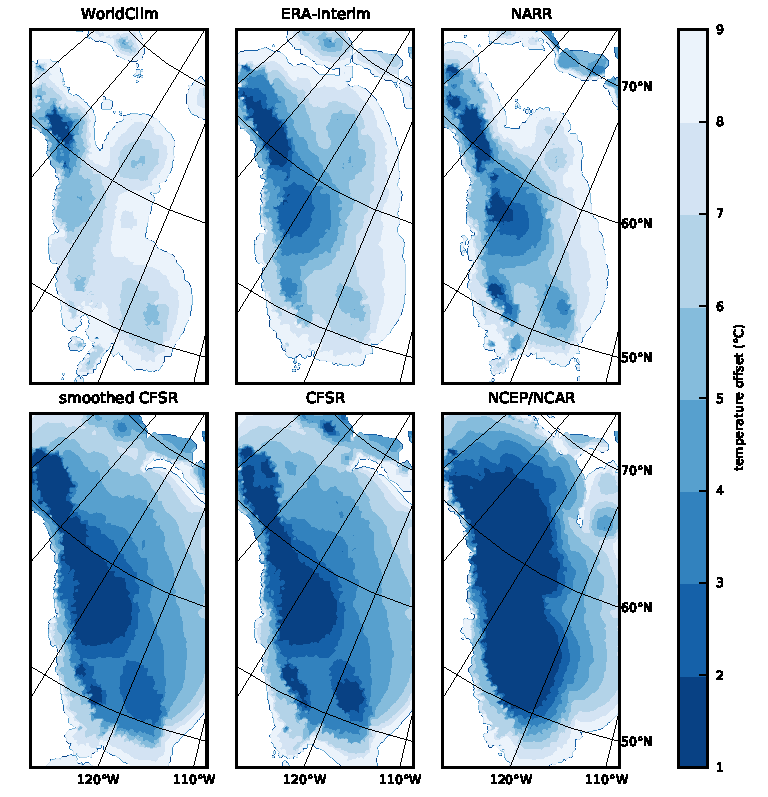
\includegraphics{cordillera-climate-extent}
  \caption{Extent of ice cover after 10\,kyr as a~function of applied temperature offsets for each climate forcing used. A~reconstructed LGM ice sheet margin by \citet{dyke-2004} (Fig.~\ref{fig:locmap}) is given for reference (black line).}
  \label{fig:extent}
\end{figure*}

% fig:cool05
\begin{figure*}
  \includegraphics{cordillera-climate-cool05}
  \caption{Ice surface topography (1\,\unit{km} contours) and velocity (\unit{m\,yr^{-1}}) after 10\,kyr under a~climate -5\,\unit{{\degree}C} colder than present for each climate forcing used.}
  \label{fig:cool05}
\end{figure*}

% fig:tempheatmap
\begin{figure}
  \includegraphics{cordillera-climate-tempheatmap}
  \caption{Density maps showing a~comparison of summer (JJA) surface air temperature data from the WorldClim climatology, against that of each reanalysis. Climate data are presented after bilinear spatial interpolation and correction for topographic differences to WorldClim data, using a lapse rate of 6\,\unit{{\degree}C\,km^{-1}}. Colour mapping is based on a~logarithmic scale. Note the cold bias of NCEP/NCAR data relative to WorldClim data.}
  \label{fig:tempheatmap}
\end{figure}

% fig:tempdiff
\begin{figure}
  \includegraphics{cordillera-climate-tempdiff}
  \caption{Summer (JJA) surface air temperature difference maps against WorldClim data, after bilinear spatial interpolation and lapse-rate correction. Note the cold bias of NCEP/NCAR data and temperature anomalies due to unresolved topographic detail.}
  \label{fig:tempdiff}
\end{figure}

% fig:precheatmap
\begin{figure}
  \includegraphics{cordillera-climate-precheatmap}
  \caption{Density maps showing a~comparison of winter (DJF) precipitation rate from the WorldClim climatology, against that of each reanalysis, after bilinear spatial interpolation. Colour mapping is based on a~logarithmic scale. Note the wet bias of all reanalysis data relative to WorldClim data.}
  \label{fig:precheatmap}
\end{figure}

% fig:precdiff
\begin{figure}
  \includegraphics{cordillera-climate-precdiff}
  \caption{Winter (DJF) precipitation rate difference maps against WorldClim data, after bilinear spatial interpolation. Note the wet bias of all reanalysis data and the large anomalies of CFSR and NCEP/NCAR data.}
  \label{fig:precdiff}
\end{figure}

% fig:oroprecip
\begin{figure}
  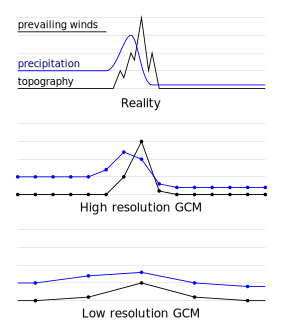
\includegraphics{cordillera-climate-oroprecip}
  \caption{Schematic representation of the orographic precipitation effect over a~mountain range. In a~GCM of low resolution, the precipitation peak appears downwind-shifted and smoother and the precipitation shadow is less pronounced than in a~high resolution GCM.}
  \label{fig:oroprecip}
\end{figure}

% fig:biatm
\begin{figure*}
  \includegraphics{cordillera-climate-biatm}
  \caption{Ice surface topography (1\,\unit{km} contours) and velocity (\unit{m\,yr^{-1}}) after 10\,kyr using ``hybrid'' climate forcing with precipitation rate from WorldClim and surface air temperature from each reanalysis (upper row), and surface air temperature from WorldClim and precipitation rate from each reanalysis (lower row). In other words, the upper row shows the effect of temperature anomalies, and the lower row the effect of precipitation anomalies, for each reanalysis, relative to WorldClim data. Each simulation uses a~-5\,\unit{{\degree}C} offset for comparison with Fig.~\ref{fig:cool05}.}
  \label{fig:biatm}
\end{figure*}

% fig:biatmbars
\begin{figure}
  \includegraphics{cordillera-climate-biatmbars}
  \caption{Effect of temperature and precipitation anomalies (separately and jointly) from each reanalysis on modelled final ice volume relative to the result of the WorldClim -5\,\unit{{\degree}C} offset simulation. Corresponding ice sheet geometries are presented in Figs.~\ref{fig:cool05} and~\ref{fig:biatm}.}
  \label{fig:biatmbars}
\end{figure}

% fig:best
\begin{figure*}
  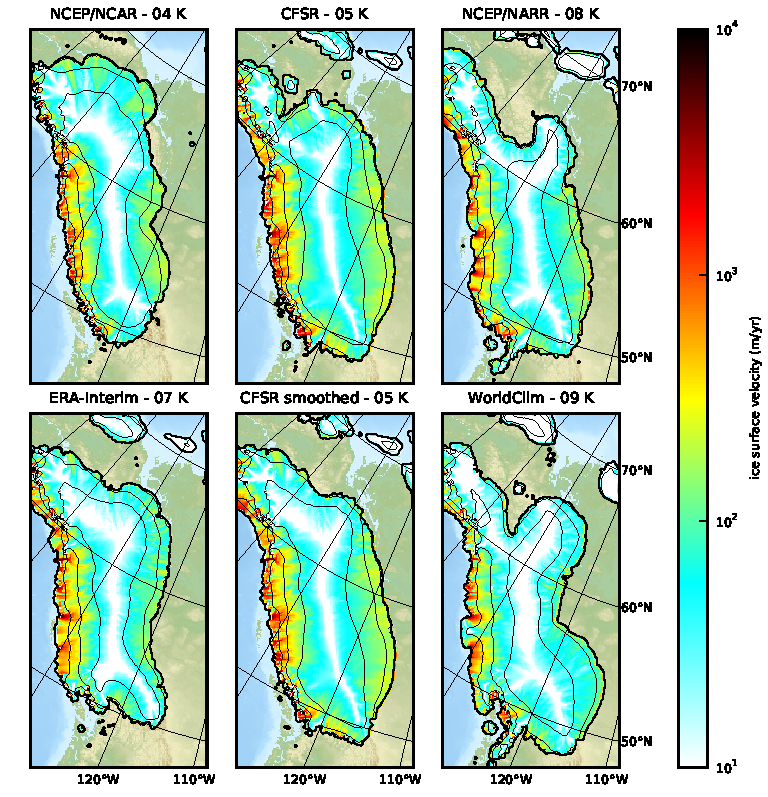
\includegraphics{cordillera-climate-best}
  \caption{Ice surface topography (1\,km contours) after 10\,kyr using temperature offsets resulting in glaciated areas of circa $2 \times 10^6\,\unit{km^2}$. A~reconstructed LGM ice sheet margin by \citet{dyke-2004} (Fig.~\ref{fig:locmap}) is given for reference (blue line).}
  \label{fig:best}
\end{figure*}

% fig:durationstack
\begin{figure}
  \includegraphics{cordillera-climate-durationstack}
  \caption{Left panel: model sensitivity to simulation length. Modelled glaciated area, using NARR forcing data, and temperature offsets from -15 to 0\,\unit{{\degree}C}, solid lines corresponding to values from -11 to -7\,\unit{{\degree}C}. Right panel: modelled ice margin corresponding to temperature offsets from -11 to -7\,\unit{{\degree}C} when total glaciated area reach the approximate size of the LGM Cordilleran ice sheet of $2 \times 10^6\,\unit{km^2}$. A~reconstructed LGM ice sheet margin by \citet{dyke-2004} (Fig.~\ref{fig:locmap}) is given for reference (grey shading). Note that shorter (and colder) simulations lead to more restrictive glaciation of the continental eastern margin but further ice extent in the maritime south-western part of the modelling domain.}
  \label{fig:durationstack}
\end{figure}

% ----------------------------------------------------------------------
\end{document}
\endinput
% ----------------------------------------------------------------------
